\subsection{Dataset}

The Cityscapes dataset is a large-scale dataset widely used for training, evaluating and benchmarking algorithms in the fields of computer vision, particularly for models used to perform semantic segmentation and instance segmentation of urban street scenes. It consists of high resolution images captured from a vehicle-mounted camera while driving through 50 different cities in Germany and neighbouring countries. The capturing apparatus is equipped with a dual lens camera for stereoscopic capability, allowing for the possibility of applying stereo vision techniques useful for tasks like depth estimation, 3D reconstruction and scene understanding. 

The images that are used in our analysis are located in the folder \textbf{leftImg8bit}. These, as the name suggests, are taken from the left lens of the stereo camera system. They form the main high-resolution images (2048$\times$1024 pixels) with an 8-bit color depth that are used for all semantic and instance segmentation tasks using this dataset. Each image is stored in a PNG file format with a size that varies between 2.0 and 2.5 MB. The images have an RGB color space, which means that there are 3 color channels for each image.

The dataset comes with two different types of image annotations:\\
\textbf{Coarse annotations:} These include a much larger set of 20,000 images with a slightly lower level of annotation detail (see Figure \ref{fig:cityscapes}(a)). We have used exclusively this set of images for our analysis as the number of samples is much more substantial and they provide more varied examples for training. 

\textbf{Fine annotations:} These provide detailed, pixel-level annotations for 5,000 images (see Figure \ref{fig:cityscapes}(b)) which include labels for 30 classes such as road, car, pedestrian, building, and traffic light. This dataset is split into 2,975 annotations for training, 500 for validation and 1,525 for testing. It is worth mentioning that the ground truth annotations for the testing set are not available to the users in order to allow for fair evaluation and benchmarking of models. Users instead need to submit their code to an online evaluation server which provides the quantitative performance metrics. 

\begin{figure}[ht]
    \centering
    \begin{subfigure}{0.45\textwidth}
        \centering
        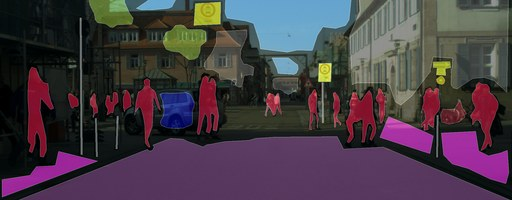
\includegraphics[width=\linewidth]{coarse_example.jpg}
        \caption{Coarse mask}
        \label{fig:sub1}
    \end{subfigure}\hfill
    \begin{subfigure}{0.45\textwidth}
        \centering
        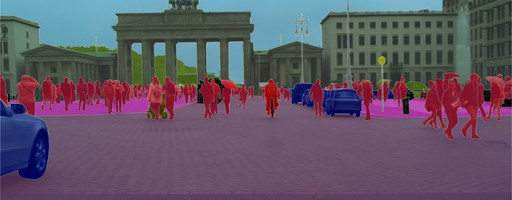
\includegraphics[width=\linewidth]{fine_example.jpg}
        \caption{Fine mask}
        \label{fig:sub2}
    \end{subfigure}
    \caption{Examples of coarse (a) and fine (b) mask annotations superimposed on the corresponding original images}
    \label{fig:cityscapes}
\end{figure}

The scenes in the CityScapes dataset represent a variety of urban settings, seasons, daylight conditions, and weather scenarios, providing robust, real-world environments for training models that need to perform under varied conditions. This dataset has been widely used in research for developing, testing and benchmarking new algorithms for computer vision tasks, gaining a place alongside datasets as iconic as ImageNet, COCO and Pascal VOC. The Cityscapes dataset can be accessed in the following address:
\begin{center}
\url{https://www.cityscapes-dataset.com}
\end{center}
Our particular approach in this study has been to start off by training a relatively simple model, that forms our baseline model, and then experiment with increasingly complex architectures. We aim to demonstrate that all these models are able to perform the task and further than that to investigate how the choice of various hyper-parameters and tweaks in architecture can affect the accuracy and performance of the models. The architectures that we have deployed in our study are briefly outlined in the section below.
